\section{Database og data access}
I dette afsnit findes dokumentation for projektets data access layer. Entity Frameworket er brugt blabla.

\subsection{Dependancy inverted design}
\todo{write stuffz!}


\subsection{Klasser og klassebeskrivelser}
På figur \ref{fig:databaseFullClass} ses klassediagrammet for database access. 

\begin{landscape}
\begin{figure}[h]
\centering
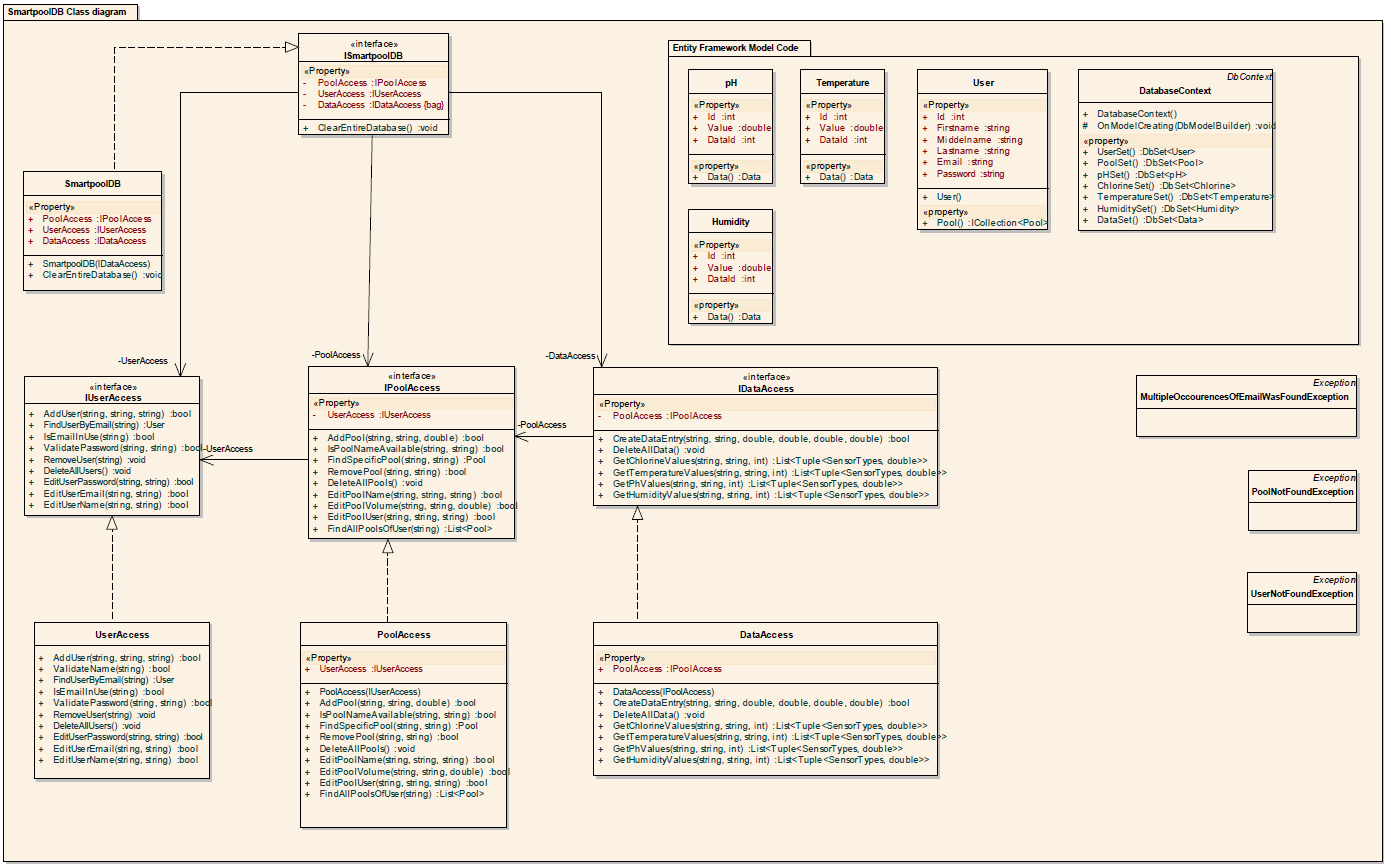
\includegraphics[width=\linewidth]{figs/implementering/databaseFullClass.PNG}
\caption{Database access klassediagram}
\label{fig:databaseFullClass}
\end{figure}
\end{landscape}


\subsubsection{DatabaseContext : DbContext}
DbContext er en del af Entity Frameworket. Som det kan ses på figur~\ref{fig:dbContextClass} arver DatabaseContext fra DbContext \cite{microsoftdbcontext} og udgør da bindeleddet fra koden til databasen.

\begin{figure}
\centering
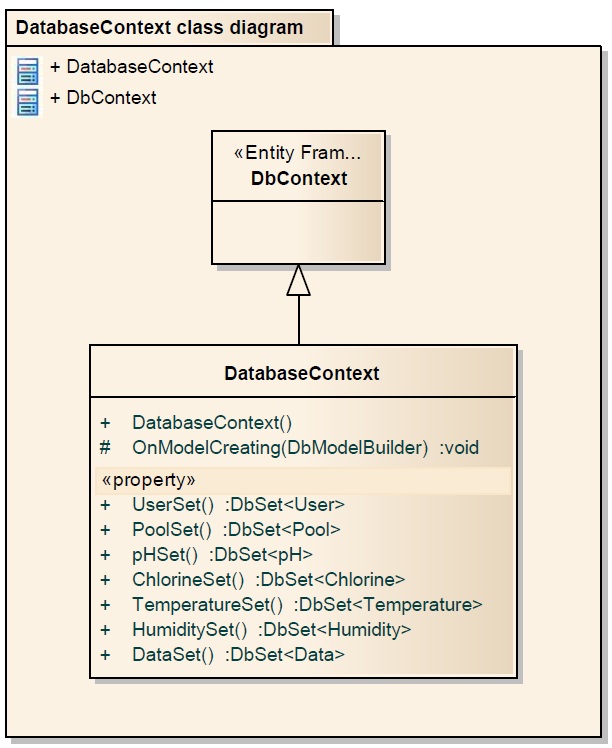
\includegraphics[width=0.3\linewidth]{figs/implementering/dbContextClass.PNG}
\caption{}
\label{fig:dbContextClass}
\end{figure}

Entities er defineret i klassen som public virtual DbSet<T> hvor typen er den specifikke entity.
DatabaseContext objektet skal oprettes når der laves en query på databasen eller sættes data ind.
På en DbSet property kan der kaldes Add(), som tilføjer en entity i den kontekst der kaldes i. Herefter skal DbContext’s SaveChanges() metode kaldes for at ændringerne skrives i databasen.

\subsubsection{SmartpoolDB}
SmartpoolDB implementerer ISmartPoolDB og står for at initialisere DataAccess, UserAccess og PoolAccess gennem deres interfaces. SmartpoolDB kan da bruge af klienter når data access funktionalitet skal bruges. I SmartpoolDB klassen findes også administratormetode der står for at slette hele databasen.

\todo{Indsæt klassediagram?}

\paragraph{Metodebeskrivelser}

\subparagraph{Constructor}\

\textit{public SmartpoolDB(IDataAccess dataAccess)}

Constructoren stå udelukkende for at initialisere SmartpoolDB-klassens pool, user -og dataaccess properties.

\subparagraph{ClearEntireDatabase}\

\textit{public void ClearEntireDatabase()}

Metoden kalder DeleteAll metoderne på dens egen properties, og derved fjernes alt data i databasen.

\paragraph{Properties}

\begin{itemize}
	\item \textit{public IPoolAccess PoolAccess { get; }}
	\item \textit{public IUserAccess UserAccess { get; }}
	\item \textit{public IDataAccess DataAccess { get; }}
\end{itemize}

\subsubsection{UserAccess}
Klassen UserAccess implementerer IUserAccess og står for at skrive og læse user records til/fra databasen.
UserAccess indeholer administrator funktionalitet til at slette alle users på databasen. Herudover står UserAccess for data editing af users samt validering af userdata før det gemmes. 

\todo{Indsæt klassediagram?}

\paragraph{Metodebeskrivelser}

\subparagraph{AddUser}\

\textit{bool AddUser(string fullname, string email, string password)}

Står for at indsætte en user i databasen. Metoden kalder IsEmailInUse samt ValidateName før der oprettes et database kontekst objekt af typen DataBaseContext. På Kontekstobjektets DbSet<User> property kaldes Add metoden med den nye User som parameter. Herefter gemmes den nye User i databasen ved at kalde SaveChanges metoden på kontekstobjektet. Adduser returnerer false hvis der er fejl i enten check på email eller fullname. Hvis det lykkes at tilføje brugeren til databasen returneres true.

\subparagraph{FindUserByEmail}\

\textit{User FindUserByEmail(string email)}

Søger i databasen efter en User med den email der angives som parameter. Det må ikke eksistere flere brugere med samme email i databasen. Søgningen udføres med et LINQ statement på databasekonteksten. Se kodeudsnit~\ref{code:finduser} .Metoden returnerer den fundne User med mindre der kastes en exception.

\begin{lstlisting}[caption=Kodeudsnit fra metoden FindUserByEmail, label=code:finduser]

...

using (var db = new DatabaseContext())
{
	var searchByEmail = from search in db.UserSet
			where search.Email.Equals(email)
			select search;

	if (searchByEmail.Count() > 1) throw new    MultipleOccourencesOfEmailWasFoundException();
	if (searchByEmail.Count() == 0) throw new UserNotFoundException();

	foundUser = searchByEmail.First();
}

...
	
\end{lstlisting}

\begin{itemize}
	\item \textit{MultipleOccourencesOfEmailWasFoundException()} - Sikkerhedsforanstaltning ved flere af samme emails.
	\item \textit{UserNotFoundException()} - Kastes hvis der ikke findes en bruger med den angivne email addresse i databasen.
\end{itemize}

\subparagraph{IsEmailInUse}\

\textit{bool IsEmailInUse(string email)}

Laver en LINQ query på databasekontekst objektet og checker om der findes en mail adresse i databasen der matcher den som er givet som parameter. Metoden returnerer false hvis mail addressen ikke er i brug og true hvis den er.

\subparagraph{ValidatePassword}\

\textit{bool ValidatePassword(string email, string password);}
Da et Fullname skal indeholde mere end et navn, checkes der her for et minimum af to navne. Hvis navnet kan godkendes returneres true, eller false.

\subparagraph{RemoveUser}\

\textit{void RemoveUser(string email)}

Checker først om en burger med email findes.
Laver en LINQ query på databasekontekst objektet. Og finder den pågældende bruger.
Brugeren fjernes ved at kalde remove på kontekstobjektets UserSet property.

\textit{db.UserSet.Remove(user)}

\subparagraph{DeleteAllUsers}\

\textit{void DeleteAllUsers()}

Bruges kun til systemtest og under udvikling.
Sletter alle brugere i databasen. Dette gøres ved at eksekvere en SQL kommando direkte på databasen. 

\begin{lstlisting}[caption=SQL injection på databasen ved sletning af brugere, label=sqlDeleteUsers]
...
using (var db = new DatabaseContext())
		{
			db.Database.ExecuteSqlCommand("DELETE [UserSet]");
		}
...	
\end{lstlisting}

\subparagraph{EditUserPassword}\

\textit{bool EditUserPassword(string email, string newPassword)}

Gør det muligt for en bruger at ændre sit password. Metoden står derudover for at sikre at det nye password ikke er en tom streng. User entitetens password property ændres gennem databasekonteksobjektet, hvorefter ændringen gemmes på databasen.
Metoden returnerer true med mindre der findes en uoverensstemmelse med enten password eller email.

\subparagraph{EditUserEmail}\

\textit{bool EditUserEmail(string email, string newEmail)}

Gør det muligt or en bruger at ændre sin email. Dette gøres gennem databasekontekst objektet. Når emailen er ændret skal brugeren benytte sig af den nye email ved et system login. \textit{Find()} metoden kaldes på kontekstobjektets UserSet property, med den ønskede brugers primærnøgle, \textit{Id}, hvorefter den pågældende User returneres. Se kodeudsnit \ref{code:idef} for eksempel på brugen af primær nøgler i entity frameworket.

\begin{lstlisting}[caption=EditUserEmail - brug af primær nøgler i Entity Framework,label=code:idef]
public bool EditUserEmail(string email, string newEmail)
{
	...
	using (var db = new DatabaseContext())
		{
			var original = db.UserSet.Find(FindUserByEmail(email).Id);
			if (original != null)
				{
					original.Email = newEmail;
					db.SaveChanges();
				}
		}
	return true;
}

\end{lstlisting}

\subparagraph{EditUserName}\

\textit{bool EditUserName(string email, string newName)}
\todo{do dis}

\paragraph{Properties}\

\todo{do dis}

\subsubsection{PoolAccess}
PoolAccess implementerer IPoolAccess og står for at skrive og læse pool records til/fra databasen. PoolAccess indeholder administrator funktionalitet til at slette alle pools på databasen. Herudover står PoolAcces for data editing af pools samt validering af pooldata før det gemmes.

\todo{Indsæt klassediagram?}

\paragraph{Metodebeskrivelser}

\subparagraph{AddPool}\

\textit{bool AddPool(string email, string name, double volume)}
\todo{do dis}

\subparagraph{IsPoolNameAvailable}\

\textit{bool IsPoolNameAvailable(string email, string name)}
\todo{do dis}

\subparagraph{FindSpecificPool}\

\textit{Pool FindSpecificPool(string email, string name)}
\todo{do dis}

\subparagraph{RemovePool}\

\textit{bool RemovePool(string email, string name)}
\todo{do dis}

\subparagraph{DeleteAllPools}\

\textit{void DeleteAllPools()}
\todo{do dis}

\subparagraph{EditPoolName}\

\textit{bool EditPoolName(string ownerEmail, string currentName, string newName)}
\todo{do dis}

\subparagraph{EditPoolVolume}\

\textit{bool EditPoolVolume(string ownerEmail, string name, double newVolume)}
\todo{do dis}

\subparagraph{EditPoolUser}\

\textit{bool EditPoolUser(string currectOwnerEmail, string name, string newUserEmail)}
\todo{do dis}


\subparagraph{FindAllPoolsOfUser}\

\textit{List<Pool> FindAllPoolsOfUser(string ownerEmail}
\todo{do dis}

\paragraph{Properties}

\subparagraph{UserAccess}\

\textit{IUserAccess UserAccess { get; set; }}


\subsubsection{DataAccess}
DataAccess implementerer IDataAccess og står for at skrive og læse data records til/fra databasen.
IDataAccess refereres af klassen SmartPoolDB


\todo{Indsæt klassediagram?}

\paragraph{Metodebeskrivelser}

\subparagraph{CreateDataEntry}\

\textit{bool CreateDataEntry(string ownerEmail, string poolName, double chlorine, double temp, double pH, double humidity)}
\todo{do dis}


\subparagraph{DeleteAllData}\

\textit{void DeleteAllData()}
\todo{do dis}

\subparagraph{GetChlorineValues}\

\textit{List<Tuple<SensorTypes, double>> GetChlorineValues(string poolOwnerEmail, string poolName, int daysToGoBack)}
\todo{do dis}

\subparagraph{GetTemperatureValues}\

\textit{List<Tuple<SensorTypes, double>> GetTemperatureValues(string poolOwnerEmail, string poolName, int daysToGoBack)}
\todo{do dis}

\subparagraph{GetPhValues}\

\textit{List<Tuple<SensorTypes, double>> GetPhValues(string poolOwnerEmail, string poolName, int daysToGoBack)}
\todo{do dis}

\subparagraph{GetHumidityValues}\

\textit{List<Tuple<SensorTypes, double>> GetHumidityValues(string poolOwnerEmail, string poolName, int daysToGoBack);}
\todo{do dis}

\paragraph{Properties}

\subparagraph{PoolAccess}\

\textit{IPoolAccess PoolAccess { get; set; }}

